\pgfplotsset{compat=1.9}

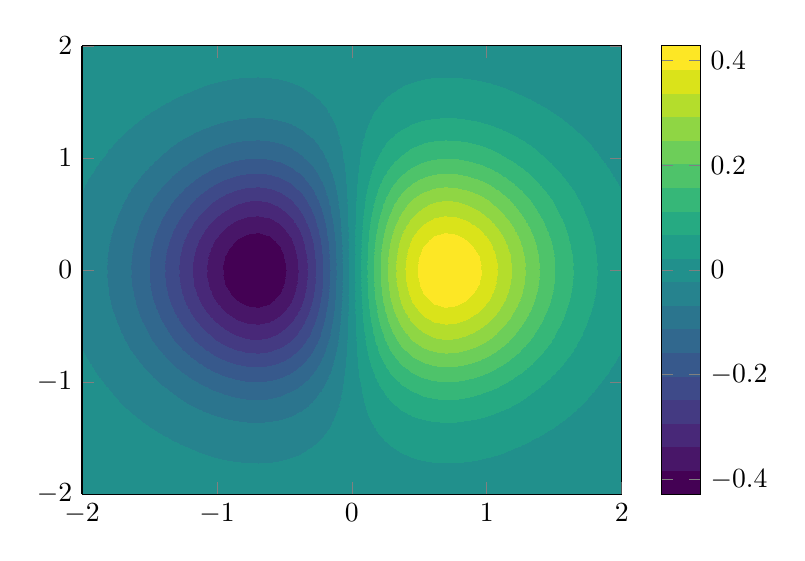
\begin{tikzpicture}
  \begin{axis}[domain=-2:2, samples=50, view={0}{90}, 
               colorbar right, colormap name = viridis]
    \addplot3[contour filled={number=19}] {exp(-x^2-y^2)*x};
  \end{axis}
\end{tikzpicture}

% Notes:
% Using less samples makes it look more rough, i.e. the contours are more jagged.
%
% ToDo:
% Maybe rename to .._ContourFill